\chapter{Relationen und Funktionen}
\section{Begriffe}
\subsection{Tupel}
Ein Tupel ist ein primitives Objekt. Zwei Tupel sind genau dann identisch wenn in beiden Tupeln das gleiche steht:
\textbf{Beispiel:} Die geordneten Paare \( (x,y) \) und \( (y,z) \) sind genau dann gleich wenn \( x = y = z \)	gilt.
\subsection{Kartesisches Produkt}
Das Kreuzprodukt zweier Mengen: A = {0,1,2}, B = {s,t}. AxB = { (0,s), (0,t), (1,s), (1,t), (2,s), (2,t) }. Das Kreuzprodukt  zweier Mengen ist wieder eine Menge und zwar eine Menge aus allen Kombinationsmöglichkeiten von Elementen aus der ersten Menge und der zweiten Menge in Tupelschreibweise geschrieben. Kann auch in einer Matrix geschrieben werden.
\section{Relationen}
\subsection{Definition}
Seien A und B zwei Mengen. Die Teilmenge R des Kreuzprodukts AxB heisst Relation zwischen A und B.
\(R \subset A \times B\).\newline
Eine Relation \(R \subset A \times A\) heisst Relation auf A. Sind \(A \) und \( B \) beliebige Mengen, so nennen wir eine Teilmenge \(R \subset A \times B. \) eine \emph{Relation} zwischen \emph{A} und \emph{B}. Sind \(a \in A \) und \(b \in B \), so sagen wir, dass \emph{a} in Relation \emph{R} zu \emph{b} steht falls \( (a, b) \in R \) ist. Steht \emph{a} in Relation \emph{R} zu \emph{b} so schreiben wir auch \emph{aRb} oder \(a \sim_R b \).

\subsection{Reflexiv}
\( \forall_a A(a): a \sim a \in R \). Jedes Element aus A steht zu sich selbst in Relation.
\begin{itemize}
	\item Die Kleiner-Gleich-Relation auf den reellen Zahlen ist reflexiv, da stets \(x \leq x \) gilt. Sie ist darüber hinaus eine Totalordnung. Gleiches gilt für die Relation \( \geq \).
	\item Die gewöhnliche Gleichheit auf den reellen Zahlen ist reflexiv, da stets \(x = x\) gilt. Sie ist darüber hinaus eine Äquivalenzrelation.
	\item Die Teilmengenbeziehung \(\subseteq \) zwischen Mengen ist reflexiv, da stets \(A \subseteq A\) gilt. Sie ist darüber hinaus eine Halbordnung.
\end{itemize}
    Um Reflexivität zu beweisen, ein Element auswählen und die Relation
    auf's erste Element anwenden. Wenn die Aussage wahr ist, steht das
    Element mit sich selbst in Beziehung.

\subsection{Symmetrisch}
\( \forall_{a,b} A: a \sim b \Rightarrow b \sim a \in R \Rightarrow (b,a) \in R \) \newline
Für alle \(a,b\) von A gilt wenn a zu b in Relation steht, dann steht auch b zu a in Relation. \newline
Wenn Person a in der selben Reihe sitzt wie Person b, sitzt Person b auch in der selben Reihe wie Person a.
\textbf{Beispiel:} \( R = \{(0,1),(0,0),(2,1),(1,0),(1,2) \} \)
    \newline Gleichheit, Ungleichheit.
	=> Wenn die Relation umgekehrt werden kann und sie immer noch gilt.
	
\subsection{Asymmetrisch}
\( \forall_{a,b} A: a \sim b \Rightarrow \neg (b \sim a) \). Für alle
    \(a,b\) aus A gilt: a ist symmetrisch zu b aber b ist nicht symmetrisch zu a.
    Wenn A \textbf{grösser als} B ist, ist B \textbf{nicht grösser als} A. Eine Asymmetrie
    ist immer auch Antisymmetrisch, da die Voraussetzung falsch ist
    (Implikation).

\subsection{Antisymmetrisch}
\(\forall_{a,b} A: a \sim b \wedge b \sim a \Rightarrow a = b \). Wenn a zu b in Relation steht und b zu a, dann ist a = b.\newline
\textbf{Beispiel:} Wenn a Vorfahre von b ist und b Vorfahre von a, dann
    sind a und b die gleiche Person.\newline
    \(\leq\),\(\geq\) sowie die Teilbarkeitsrelation \(x | y\)

\subsection{Transitiv}
\( \forall_{a,b,c} A: a \sim b \wedge b \sim c \Rightarrow a \sim c \).
    Wenn a in Relation zu b steht und b in Relation zu c, dann steht auch a
    zu c in Relation.\newline
    \textbf{Beispiel:} \(<,>,=,\subset, A \Rightarrow B und B \Rightarrow
    C, = A \Rightarrow C\)\newline
    \( R = \{(a,b),(b,a) \}\) = nicht transitiv! \newline
    \( R = \{(a,b),(b,a),(a,a),(b,b) \}\) = transitiv!

\subsection{Äquivalenzrelation}
Eine Relation die reflexiv, symmetrisch und transitiv ist, heisst
    Äquivalenzrelation.\newline
    Eine Äquivalenzklasse sind die disjunkten Mengen der Äquivalenzrelation, also alle Mengen, die zwar die gleiche Eigenschaft haben, ansonsten aber nichts miteinander gemeinsam haben (zb. alle binären Zahlen mit der gleichen Anzahl der Ziffer 1).

\subsection{Halbordnung}
Die Relation R wird als Halbordnung bezeichnet, falls sie transitiv,
    reflexiv sowie antisymmetrisch ist.\newline
    \(A \subset B\): Bei zwei Mengen, muss nicht zwingenderweise eine Menge
    eine Teilmenge der anderen sein.

\subsection{Totalordnung}
Gilt zusätzlich zur \emph{Halbordnung} noch für alle \(a,b \in A\)
    stets \(a \sim b \vee b \sim a\) so ist R eine \emph{Ordnung} auf A. =>
    transitiv, irreflexiv und antisymmetrisch.

\subsection{Beispiele} % (fold)
\label{sub:beispiele}
\begin{longtable}{c|l}
	\(=\) & reflexiv, transitiv, symmetrisch, antisymmetrisch, ist eine Äquivalenzrelation \\ \hline
	\(\geq,\leq\) & reflexiv, transitiv, antisymmetrisch, ist eine Totalordnung \\ \hline
	\(<,>\) & asymmetrisch, transitiv, nicht antisymmetrisch, nicht relativ, nicht total
\end{longtable}
% subsection beispiele (end)
	
\section{Funktionen}
\subsection{Allgemein}
    Eindeutige zweiteillige Relationen. Eine beliebige Teilmenge \(f
    \subset X \times Y \), \(f: x \rightarrow y \).\newline
    \begin{itemize}
      \item Domain: A, \(f(x)\), dom, Urbild, Definitionsbereich
      \item Image: B, y, Im(...), Bild, Zielmenge, Wertebereich
    \end{itemize}


\subsection{Injektiv}
\begin{wrapfigure}{r}{0.4\textwidth}
  \vspace{-20pt}
  \begin{center}
    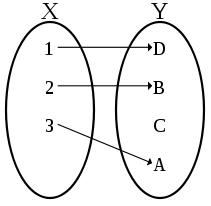
\includegraphics[width=0.25\textwidth]{Bilder/injektiv}
  \end{center}
  \vspace{-20pt}
  \caption{Injektivität}
  \vspace{-10pt}
\end{wrapfigure}
Injektivität oder \textbf{Linkseindeutigkeit} besagt, dass jedes
    Element der Zielmenge \textbf{höchstens} einmal als Funktionswert angenommen
    wird. Kein Wert der Zielmenge wird mehrfach angenommen. Dabei darf die Domain kleiner als die Zielmenge sein.\newline
\( \forall_{x,y} \in dom(F): (F(x) = F(y) \Rightarrow x = y) \)
\newline

\subsection{Surjektiv}
\begin{wrapfigure}{r}{0.4\textwidth}
  \vspace{-20pt}
  \begin{center}
    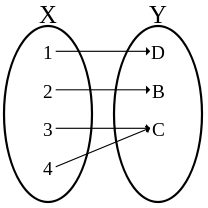
\includegraphics[width=0.25\textwidth]{Bilder/surjektiv}
  \end{center}
  \vspace{-20pt}
  \caption{Surjektivität}
  \vspace{-10pt}
\end{wrapfigure}

Surjektivität oder \textbf{Rechtstotalität} bedeutet, dass jedes
    Element der Zielmenge mindestens einmal als Funktionswert angenommen
    wird, also mindestens ein Urbild hat. Jedes Element von Y wird
    angenommen.
\(F: x \rightarrow y\) \newline
\(F: \mathbb{N} \rightarrow \mathbb{N}: F(n) = n^2 \) injektiv, nicht surjektiv\newline
\(G: \mathbb{R} \rightarrow \mathbb{R}: G(x) = x^2 \) nicht injektiv, nicht surjektiv\newline
\(F: X \rightarrow Y:\) jedes Element von y wird erreicht auch: \(im(F) =y\)

\subsection{Bijektiv}
\begin{wrapfigure}{r}{0.4\textwidth}
  \vspace{-20pt}
  \begin{center}
    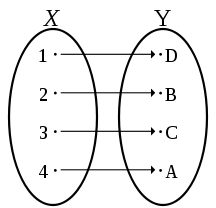
\includegraphics[width=0.25\textwidth]{Bilder/bijektiv}
  \end{center}
  \vspace{-20pt}
  \caption{Bijektivität}
  \vspace{-10pt}
\end{wrapfigure}
Eine Funktion ist bijektiv (oder \emph{umkehrbar eindeutig auf} oder
    \emph{eineindeutig auf}), wenn sie sowohl injektiv (kein Wert der
    Zielmenge wird mehrfach angenommen) als auch surjektiv (jeder Wert der
    Zielmenge wird angenommen) ist. Insgesamt heißt das, es findet eine
    vollständige Paarbildung zwischen den Elementen von Definitionsmenge
    und Zielmenge statt. Nur Bijektionen behandeln ihren Definitionsbereich
    und ihren Wertebereich symmetrisch, sodass eine bijektive Funktion
    immer eine Umkehrfunktion hat bzw. invertierbar ist. "Für jedes A gibt
    es ein B".
\begin{align*}
	F \circ G \circ H &= F(G(H(x))) &&\\
	&= F \circ (G \circ H) &&\\
	&= (F \circ G) \circ H &&
\end{align*}
\(G\circ F: x \rightarrow z\) und \(G \circ F(x):= G(F(X))\).\newline
\((x,y) \in F = F(x)=y\).

\subsection{Äquivalenzklassen}
Ist $A$ eine Menge und $\sim$ eine Äquivalenzrelation auf $A$, dann sind folgende Aussagen äquivalent:
\begin{enumerate}
	\item $\sim$ ist eine Äquivalenzrelation auf $A$
	\item Es gibt eine Funktion $F : A \rightarrow \powerset (A)$, so dass für alle $x, y \in A$ 
	$$x \sim y \Leftrightarrow F(x) = F(y)$$
	gilt.
\end{enumerate}
Ist $F$ eine Funktion wie in 2., dann ist das eine Äquivalenzklasse von $\sim$. 
\begin{bsp}
Schüler, die alle in der gleichen Reihe sitzen, haben als ihre Äquivalenzklasse diese Reihe.
\end{bsp}

\subsection{Umkehrabbildung}
\begin{align*}
	h(-z) &= z\\
	h^{-1}(z) &= -z	
\end{align*}